\chapter{Analisi e validazione dei risultati}
\label{analisi}

\section{Analisi temporale}
Questo tipo di analisi è stata effettuata al fine di determinare la frequenza massima entro la quale il microcontrollore è in grado di eseguire tutte le operazioni basilari, rappresentate in Fig.\ref{fig:temp}. Ovvero per rispondere alla seguente domanda:
\begin{quotation}
	\textit{Qual'è la finestra temporale minima sufficiente a garantire 
		che il microcontrollore sia in grado di eseguire correttamente le funzioni basilari? }
\end{quotation}
Dove per funzioni basilari si intendono le operazioni di:
\begin{itemize}
	\item \textbf{Lettura} dei dati grezzi dall'IMU tramite, indicato con $T_{RX\_I2C}$
	\item \textbf{Trasmissione} dei dati verso il modulo \textit{App} (si veda\ref{livello_moduli}), indicato con $T_{TX\_USB}$
\end{itemize}


 \begin{figure}[H]  
	\centering 
	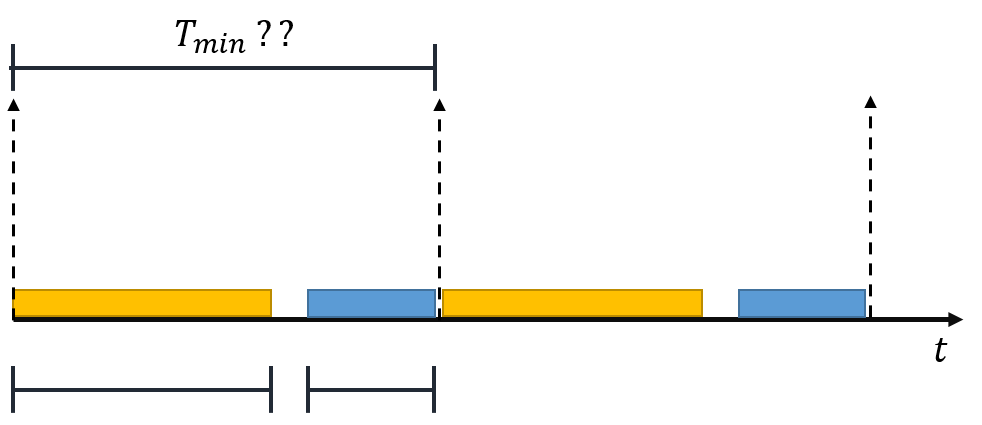
\includegraphics[scale=0.35 ]{analisi/temp1.png}
	\caption{Rappresentazione della finestra temporale minima per eseguire le operazioni basilari}
	\label{fig:temp}
\end{figure}

Per far ciò è opportuno analizzare singolarmente i due tempi, considerando le relative informazioni e la velocità del mezzo di comunicazione.\\

\subsection{Analisi del tempo di lettura dei dati grezzi dall'IMU}
\label{analisii2c}
Le informazioni riguardanti le grandezze fisiche misurate dai sensori integrati nell'IMU (Cap.\ref{tecnologie}), tramite I2C (Cap.\ref{imp_i2c}), su un singolo asse del \textit{b-frame} (Cap.\ref{modello_di_misura}), sono rappresentate attraverso \textbf{16 bit}.\\
Di conseguenza il tempo di lettura $T_{RX\_I2C}$ è dato dalla seguene equazione:
\begin{equation}
\label{eq:ti2c}
	T_{RX\_I2C} = N_{sensori} \cdot N_{assi} \cdot T_{i\_asse}
\end{equation}
Dove:
\begin{itemize}
	\item $N_{sensori}$ sono il numero di sensori utilizzati 
	\item $N_{assi}$ sono il numero di assi utilizzati dai sensori
	\item $ T_{i\_asse}$ è il tempo di lettura del singolo asse
\end{itemize}

Dunque il problema si riduce alla determinazione di $ T_{i\_asse}$. Per come è implementata l'IMU, la lettura di un singolo asse si completa leggendo due registri da \textbf{8 bit}.
\begin{equation}
 T_{i\_asse} = 2 \cdot T_{RX\_8bit}
\end{equation}

Per stimare $T_{RX\_8bit}$ si è programmato il microcontrollore in modo tale da leggere 1000 volte un registro da 8 bit e misurare il tempo trascorso leggendo i \textit{tick} di sistema. Per il codice si rimanda alla lettura dell'App.\ref{app:stimai2c}.\\ 
Eseguendo il test svariate volte, si è osservato che il tempo necessario per leggere 1000 volte un registro da 8 bit è pari a $101 ms$. 
Questo implica un \textit{goodput} di $80 Kb/s$ pari al $20\%$ della capacità del canale di comunicazione, che risulta essere $400 Kb/s$ essendo un I2C in \textit{fast-mode}. Questo calo è dovuto a numerosi fattori tra i quali l'overhead del protocollo e la velocità del microcontrollore.\\
Quindi andando a sostituire il valore stimato per la lettura di 8 bit nell'Eq.\ref{eq:ti2c} si ottiene, per l'uso dell'IMU a 9DOF:
\begin{equation}
T_{RX\_I2C} = 3 \cdot 3 \cdot (2 \cdot T_{RX\_8bit}) = 3 \cdot 3 \cdot (2 \cdot 101\mu s )= 1,8 ms
\end{equation}
Mentre per l'uso a 6DOF:
\begin{equation}
T_{RX\_I2C} = 3 \cdot 2 \cdot (2 \cdot T_{RX\_8bit}) = 3 \cdot 2 \cdot (2 \cdot 101\mu s )= 1,2 ms
\end{equation}


\subsection{Analisi del tempo di trasmissione dei dati tramite USB}
\label{analisiusb}
Il tempo necessario per trasmettere un pacchetto, dal modulo \textit{microcontrollore} al modulo \textit{App} (Cap.\ref{livello_sottosistemi}) mediante il canale USB (Cap.\ref{imp_usbcdc}), è dato dalla seguente equazione:
\begin{equation}
\label{tx_usb}
T_{TX\_USB}=  \frac{dim(pack)}{goodput}
\end{equation}
Per stimare il \textit{goodput} si è programmato il microcontrollore in modo da inviare 1000 volte un pacchetto contente un \textit{id} (univoco e incrementale) e un contatore incrementato quando il buffer di trasmissione risulta essere ancora occupato. Per il codice si rimanda alla lettura dell'App.\ref{app:stimausb}.
Eseguendo il test numerose volte, si è osservato che il tempo necessario per trasmettere 1000 pacchetti, per un totale di 8574 Bytes, è di circa $57 ms$. 
Questo implica un \textit{goodput} di $1,2 Mb/s$ pari al $10\%$ della capacità del canale di comunicazione che, essendo un USB 1.1, risulta essere $12 Mb/s$. Ancora una volta questo calo di prestazioni è dovuto a numerosi fattori tra i quali l'overhead del protocollo, l'implementazione della libreria STM utilizzata e la velocità del microcontrollore.\\
Più complicato è il discorso riguardante la dimensione dei pacchetti da trasmettere, questi infatti sono strettamente correlati a:
 \begin{itemize}
 	\item \textbf{La modalità di computazione} selezionata (Cap.\ref{computationMode})
 	\item \textbf{Il numero di sensori} utilizzati
 	\item \textbf{La codifica} dell'informazione
  \end{itemize}

Con riferimento alle possibili combinazioni dei fattori precedenti e alle rispettive strutture dei pacchetti, dettagliate nel Cap.\ref{tcm}, si hanno le seguenti dimensioni: 
\begin{enumerate}
	\item \textbf{LCM}:
		\begin{enumerate}
		\item \textit{6DOF} = 48 Bytes
		\item \textit{9DOF} = 63 Bytes
		\end{enumerate}
	\item \textbf{HCM} = 21 Bytes
	\item \textbf{TCM}:
			\begin{enumerate}
			\item \textit{6DOF} = 63 Bytes
			\item \textit{9DOF} = 84 Bytes
			\end{enumerate}
\end{enumerate}

Sostituendo questi valori e la stima del \textit{goodput} del canale all'Eq.\ref{tx_usb}, si ottengono le stime dei diversi tempi di trasmissione:

\begin{enumerate}
	\item \textbf{LCM}:
	\begin{enumerate}
		\item \textit{6DOF}: $ T_{TX\_USB}=  \frac{48 Bytes}{1,2 Mbit/s} = 0,32 ms $
		\item \textit{9DOF} : $ T_{TX\_USB}=  \frac{63 Bytes}{1,2 Mbit/s} = 0,42 ms $
	\end{enumerate}
	\item \textbf{HCM} : $ T_{TX\_USB}=  \frac{21 Bytes}{1,2 Mbit/s} = 0,16 ms $
	
	\item \textbf{TCM}:
	\begin{enumerate}
		\item \textit{6DOF} : $ T_{TX\_USB}=  \frac{63 Bytes}{1,2 Mbit/s} = 0,42 ms $
		\item \textit{9DOF} : $ T_{TX\_USB}=  \frac{84 Bytes}{1,2 Mbit/s} = 0,56 ms $
	\end{enumerate}
\end{enumerate}



\subsection{Conclusioni analisi temporale}
Sommando i tempi stimati nei paragrafi precedenti (Cap.\ref{analisii2c} e Cap.\ref{analisiusb}), si ottengono le diverse finestre temporali minime affinché, il microcontrollore riesca a completare le funzioni basilari:

\begin{enumerate}
	\item \textbf{LCM}:
	\begin{enumerate}
		\item \textit{6DOF}: $T_{min} = T_{RX\_I2C} + T_{TX\_USB} = 1,2 ms + 0,32 ms = 1,52 ms $
		\item \textit{9DOF} : $ T_{min} = T_{RX\_I2C} + T_{TX\_USB} = 1,8 ms + 0,42 ms = 2,22 ms $
	\end{enumerate}
	\item \textbf{HCM} :
		\begin{enumerate}
		\item \textit{6DOF}: $T_{min} = T_{RX\_I2C} + T_{TX\_USB} = 1,2 ms + 0,16 ms = 1,36 ms $
		\item \textit{9DOF} : $ T_{min} = T_{RX\_I2C} + T_{TX\_USB} = 1,8 ms + 0,16 ms = 1,96 ms $
	\end{enumerate}
	\item \textbf{TCM}:
	\begin{enumerate}
		\item \textit{6DOF} : $ T_{min} = T_{RX\_I2C} + T_{TX\_USB} = 1,2 ms + 0,42 ms = 1,62 ms $
		\item \textit{9DOF} : $T_{min} = T_{RX\_I2C} + T_{TX\_USB} = 1,8 ms + 0,56 ms = 2,36 ms $
	\end{enumerate}
\end{enumerate}
 
Che corrispondono alle seguenti frequenze di lavoro massime:

\begin{enumerate}
	\item \textbf{LCM}:
	\begin{enumerate}
		\item \textit{6DOF}: $f = 657 Hz $
		\item \textit{9DOF} : $f = 450 Hz $
	\end{enumerate}
	\item \textbf{HCM} :
	\begin{enumerate}
		\item \textit{6DOF}: $f = 735 Hz $
		\item \textit{9DOF} : $f = 510 Hz $
	\end{enumerate}
	\item \textbf{TCM}:
	\begin{enumerate}
		\item \textit{6DOF} : $f = 617 Hz $
		\item \textit{9DOF} : $f = 423 Hz $
	\end{enumerate}
\end{enumerate}

 Da notare che tali stime non tengono conto di alcune latenze legate all'esecuzione del codice all'interno del microprocessore, per questo motivo si ritiene opportuno sovrastimare le finestre temporali e sottostimare le frequenze massime, in modo da avere margini di sicurezza e stabilità maggiori.

